\documentclass{article}

\usepackage{rotating}
\usepackage{graphicx}
\usepackage[utf]{inputenc}
\usepackage{url}

%8.5 pages is 60% 14 (max) pages
\title{A Framework for Coping with API Evolution in a Software Ecosystem Setting}


\begin{document}


\author{John Burchell \qquad William Granli \\
		john.a.burchell@gmail.com \qquad william.granli@gmail.com \\
		Computer Science and Engineering  \\
		University of Gothenburg }

\maketitle
\section{Executive Summary}
This report presents a plan for how to develop and distribute a framework for designing and improving Application Programming Interfaces (APIs) in the context of software evolution and software ecosystems. \smallskip

The research behind the framework has been made through reviewing existing literature, and through analysing changes between  different versions on an industry API. The main way of assessing the API has been through measuring the impact it has on its ecosystem. The development of the framework has been supported by a solid technology roadmap, dissemination plan and impact assessment. \smallskip

The findings of our initial studies show that the changes to APIs have negative effects, and that they primarily affect the users of the API. They also show that modifications to APIs heavily influence the ecosystem. \smallskip

With this report we conclude that the improvement potential to the current ways of designing APIs is huge. This can especially be achieved by weighing in the needs of the whole ecosystem when designing APIs. We also conclude that there is a large need for a framework such as the one we are proposing, and that it could lead to major improvements in areas such as the open-source community and in web development. The three most important benefits of our paper are: 

\begin{itemize}
\item Increased usability APIs
\item Reduced negative impacts when changing APIs
\item A software ecosystem existing in symbiosis
\end{itemize}

One limitation to this report is that the development of the framework has not started yet, and that only the initial studies have been started. Another limitation is that the no extensive research on whether or not companies have the desire spend resources that do not have an immediate impact on their revenue. 

\section{Problem Formulation}
This section will describe the problem that we are trying to solve, why it is important and what related products exist on the market today.

\subsection{Description of the Problem}

As the software industry and the open source movement steadily grow, the number of publicly available APIs is increasing. APIs can improve development speed \cite{stylos2006comparing}, improve software quality \cite{stylos2006comparing} and can increase software reusability \cite{afonso2012evaluating}. There is a consensus among literature and experts that modifications to deployed APIs can have negative impacts on the users of the API \cite{google_talk} \cite{mcdonnell2013empirical} \cite{robbes2012developers} \cite{henning2007api}. The main reason is that it will require the users to update the code using the API, thus causing a disruption in the application's software ecosystem \cite{messerschmitt2005software}. The most common changes to APIs occur from refactoring \cite{dig2005role} \cite{xing2006refactoring}.

\subsection{Research Question}
\begin{itemize}
\item How can effective changes be made to deployed APIs with minimal impact upon the ecosystem in which the API is utilised?
\end{itemize}

%Highlight problem and who it's for here.
\subsection{Why is this important?}
Having a stable and well designed API is vital to the success of a company or product, especially if they are built around a particular API. For example, a study on the impact of reliable APIs was undertaken in the Android ecosystem \cite{mcdonnell2013empirical}. The study aimed to discover if APIs with high rates of faults affected the success of an application. The study found that the 50 least popular applications had APIs which were 500\% more error prone, ultimately concluding that there is indeed a correlation between API stability and application success \cite{mcdonnell2013empirical}. \smallskip

Due to the negative implications that modifications to APIs cause for users, it is important to understand why changes occur. If the most common pitfalls are known before the development of new APIs begin, these mistakes could be mitigated. Likewise, if common dangers of changes to existing APIs are fully studied and understood, informed changes can be made to lessen the affect on the users. Furthermore, industry and academia can use these lessons learned to create, or enhance existing best practices of API design.\smallskip

Given that software is prevalent in our lives, it is likely that poor API design changes have affected our lives at some point. One could therefore argue that this problem is important to everyone; customers, businesses and developers. \smallskip

%This needs fluffing
Our solution is to provide a set of guidelines, or framework with which to follow when making changes to APIs. The framework will prioritise business motives and needs when tackling design decisions. The framework will also take into account the business need, not only of the organisation which owns the API, but the business needs of all organisations existing in the ecosystem.

\subsection{Related Products}
Exhaustive research has found that there exists very few similar solutions similar to our own. While there are countless books related to the subject, very few actually aim to address the needs of business and customers; they are primarily focused on the developer. \smallskip

Apiary \cite{Apiary} is a popular online API design service. Apiary focuses on a collaborative approach to creating APIs, the tool offers the ability to work with between 5 and 50 contributors on a single project. The unique part of this tool is that it provides a ``mock" API by which customers, developers or anyone with access can work with. This stage allows quick prototyping and testing of an API before any real coding has taken place. The tool, while useful, doesn't aim to solve the problem of handling changes to APIs but is instead a good platform to quickly prototype ideas.

Mashery \cite{Mashery} provide a more business oriented approach to API development. They offer a wide variety of services with API management being one of them. Quoting their website, they:

\begin{itemize}
\item Increase productivity through uniformity and accessibility of data
\item Develop better customer experiences faster, for mobile and web-based applications
\item Achieve real-time data exchange between platforms and applications
\item Enhance visibility into data consumption to optimise APIs
\end{itemize}

While Mashery have a more business oriented approach, they do not offer anything resembling a framework for both business and developers to use when making API design decisions.

\section{Plan and Roadmap}
As mentioned in Section 2, the effects modifications to APIs have on the platform’s ecosystem are explored as being negative. However, there are no existing systematic guidelines or frameworks that take the ecosystem into account for how to best modify an API. Our proposed process for creating such a framework can be seen in Figure \ref{fig:roadmap}. This is an initial version of the roadmap \cite{phaal2004technology}, and it is advised that it is updated during the process. The main reason for this is that it is important to adapt to changes in the market, and if new needs are identified, the strategy should be redesigned to meet them. 

\subsection{Designing the Roadmap}
The roadmap was developed using the standard T-Plan process \cite{phaal2004technology}. As such, identifying the market need was done as a part of the initial step. Following that, the products and technology needed to fill that gap were identified. As a final step the dependencies and ordering of the identified activities were sorted out which resulted in the current version of the roadmap. An overview of the process used to create the roadmap can be seen in Table \ref{tab:proc}

\begin{table}[ht]
\centering
\begin{tabular}[ht]{|c|l|l|}
\hline
\textbf{\#} & \textbf{Phase} & \textbf{Description} \\
\hline
1 & External & Identify the market needs \\
\hline
2 & Products & Identify required studies \& frameworks \\
\hline
3 & Technology & Identify required knowledge \\
\hline
4 & Organise & Identify what pull factors require which push factors \\
\hline
\end{tabular}
\caption{Roadmap Design Process}
\label{tab:proc}
\end{table}

\subsection{Knowledge Development}
Since we have made the assessment that the market need will to remain relatively stable, careful research is essential to be able to deliver a product that meets the market needs. The primary method of performing the initial study, to be able to improve knowledge, will be through studying the existing literature. The reason for this is that three fields, API design, software evolution and software ecosystems, are currently well-explored, but the correlation and relationship between them has not yet been identified. Therefore, these fields will be explored in literature and a set of ``best practices" will be gathered from each of them. \smallskip

In addition to the literature review, a case study will be conducted to gather information from a company leading its field. The goal of the data collection performed in the case study will also be to gather a set of best practices for each of the three fields. To determine these best practices, an analysis of the companies current API and a future API will be performed. The changes between the two versions of the company's platform API will be of great significance and it is from these changes that we will base some of our best practices upon. \smallskip

\subsection{Implementing the Framework}
In order to collate as much existing knowledge and research as possible, a thorough, extensive literature review will be conducted. This will be complimented by a case study which is shall be performed in conjunction with the previously mentioned case company. The results of both the review and the case study will be analysed and compared. A set of best practices, based on the data collected in the review and case study, will be used to create the basis of the framework that will make up our best practices. Bringing in important factors from each of the three fields in the discussion is of the highest importance. The goal of this phase is therefore to create an Minimum Viable Product (MVP) that can be adopted and evaluated at the case company. \smallskip

Once this information has been fully analysed and documented, with the best practices found, the framework can be created in full. The framework needs to be language agnostic and apply to no specific technical area, rather it should be applicable to all.

\subsection{Adoption and Evaluation}
The final stage of the roadmap will be performed using an iterative approach, where the MVP will be continuously evaluated and improved at the case company. The primary result of evaluating the success of the framework will be to measure if there is any visible reduction in the amount of negative effects that changes to an API has on its ecosystem, while retaining the original complexity and usability before the changes were made. \smallskip

To ease the adoption process, a series of tests and evaluations will be performed on pilot studies. The goal of these pilot studies would be to verify and improve the best practices. For example, we will perform an analysis of an exist API and it's changes against an existing framework. We will then apply our framework and best practices to see if our framework suggests better and more robust changes, taking into account the affects of these changes on the ecosystem. Feedback will then be collected from the company who owns the API based on our frameworks suggested changes. This will be done to determine if our suggested changes are achieving the same goals as their changes would have done.

\begin{sidewaysfigure}[p]
\centering
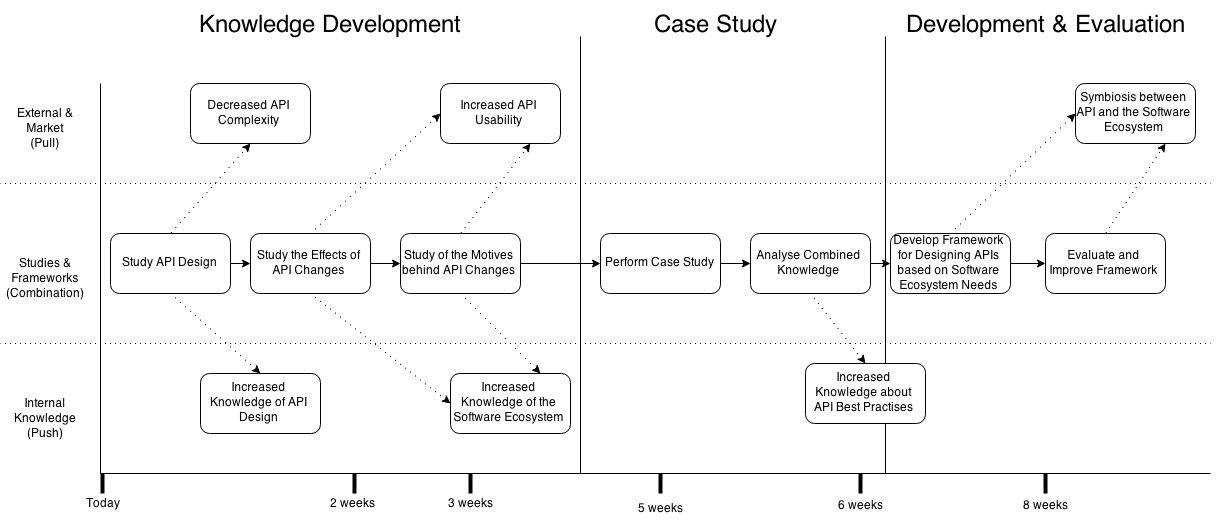
\includegraphics[width=220mm]{RoadMap.png}
\caption{The full lines denote in which way the organisation should ``logically'' view the roadmap. The dotted lines denote that one activity will lead to another. }
\label{fig:roadmap}
\end{sidewaysfigure}
%TODO: Add colours+graphix so that it's innovative and stuff

\section{Dissemination Plan, 2p}
This section will describe the dissemination plan for our framework. 

\subsection{End-users}

Two immediate end-users of our framework have been identified, 1) open-source projects and 2) web development APIs. Open-source projects have been identified as potential users of our API as they generally have a good-will mindset when it comes to furthering and helping to improve the software engineering industry. Generally speaking, most open-source developers do no prioritise making a profit from their work, instead, they focus on delivering a product that is as complete and functional as possible. The open-source community is a well established and has existed for a long time, with a long tradition of autonomy, it can be said that they care about the well-being of their software ecosystems. 

The second area where this could have an especially great impact would be in the area of web development APIs. Web APIs are widely used by vast amount of developers, performing many varied tasks. The web is a constantly evolving and expanding market, as such many companies rise and fall based on the success of their API. Therefore, it's not surprising that changes to a web API have significant impacts on the ecosystems of the systems. The toolchain in web development is usually referred to as a ``stack" which literally is a set of frameworks and APIs that you use together to develop your application.

\subsection{Presentation and Communication}
The most appropriate method of conveying our message and findings would be through the research community. The initial studies that will be conducted (as mentioned in Section 3) will lead to a number of published research papers. These papers will be used to generate awareness and attention of our framework and the successes that it can bring. The papers may propagate research and act as a stepping stone for other research. Other researchers could quite easily build upon the research which we have conducted. The outcome of which would only help our cause; to improve APIs everywhere. 

In addition to reaching out to the research community, conferences, especially those related to web development, would be targeted for publication. One example of such a conference is JDays, where many APIs that are developed in JavaScript are discussed. The main reason for targeting such conferences is that, generally speaking, these types of conferences tend to attract the prominent figures in a particular industry or a narrower aspect of it. Bringing this to the awareness of these key players would help to create further awareness and publicity of the research, and by association, the best practices that we shall develop.

The last way of presenting our framework would be through directly targeting a set of companies that operate in the same software ecosystem. One example of that would be to target a company which develops a game engine, and at the same time contact the most prominent game developers which utilise this game engine. If the company developing the game engine realises that there is large interest from the main users of their API, it is much more likely that they would be interested in using our API. 


\section{Impact Assessment}
This section will describe the impact that our framework will have. 

\subsection{Background}
The most significant impact of our new API framework would be that it could potentially transform the way companies and organisations motivate their design decisions for APIs. Today's software engineering companies mainly take into account their own agendas, and APIs are changed for refactoring reasons, such as name changes, or to reduce complexity. The most important factor when designing or changing APIs is, however, how the changes will impact the users of the API and how their needs are being met. In the recent years, this has been realised by the software engineering industry. As a result, the consensus is to have less deprecations when changing APIs and thus these changes have had their impact upon users reduced. 

\subsection{Impact on Technology and State of the Art}
The next step that we propose the industry takes, is to weigh the needs of the whole ecosystem and not just the immediate needs of the user when creating or modifying APIs. By doing this, a more homogeneous environment would be possible where API platforms and API users can change their code simultaneously. For example, it would have the potential to reduce the risks taken when deprecating methods as users and developers would be able to communicate their needs effectively. The impact of this could even be that companies begin changing and improving their APIs with the view of helping the ecosystem instead of purely their own immediate needs. This would have the potential to cause a a domino effect in the ecosystem which would hopefully spread to other ecosystems and ultimately would become a part of their overall software design process. 

More importantly, the companies themselves will likely benefit from such a framework. Potentially, the framework could allow companies to develop APIs, and therefore software, quickly and more efficiently thus increasing their development speed. Furthermore, the framework could help companies make changes to existing APIs to have fewer side effects within their ecosystems, for example, it could allow companies to communicate more easily with their users when making changes to the APIs that they are using. This could mean that companies could make changes more frequently with less side effects.

\subsection{Impact on Society}
Companies are not the only entity that could benefit from the this framework. If companies begin developing their APIs to fit the needs of ecosystems, it would not only have a great impact on these specific isolated environments; it would develop the whole software engineering industry. Therefore, the impact on society is potentially huge. Given that software is used by everyone, daily, improving software overall could improve peoples quality of life.

In modern software development, very few applications are written without the use of APIs. The consequence of which means, if APIs are designed more thoroughly, software performance is likely to rise. It might be difficult to envision that companies would actually spend resources to help their ecosystem without seeing and direct and immediate improvements for themselves. However, examples of where similar changes are happening can already be found today. One example is Ericsson. Ericsson are spending a lot of resources to develop open-source software such as Eclipse and Papyrus. The improvement of this software helps Ericsson directly, as they are using the software themselves. However, by improving open source software, they inadvertently help anyone else who uses this software. If this trend were to catch on, it could potentially lead to a world where all software has higher quality and is developed faster. 

\section{Summary}
The knowledge gained from the course has had both immediate and long term benefits. Immediately, we were able to use the information regarding finding research topics, collaborating with industry and performing research. These topics were invaluable for us when it came to finding a research topic and company for our thesis. In regards to the long term value, information for working at a company or in a professional environment will undoubtedly be of use for us. 

The guest lectures were very useful as we received first hand accounts of how research is conducted within industry. This was particularly valuable given how our our solution is heavily involved with research and academia. If either of us wish to pursue a career in research, we now have some idea of what it would require and to some extent what it might be like to do so.

The second guest lecture was also of great help when for this report. The methods and ideas presented were vital in helping us generate ideas and solutions to our given problem.

The course has thought us how to apply the theoretical knowledge we have in a business setting. Other courses, such as pure programming courses, only teach you how to do something in theory but not how to use the skills in projects or at a company. This course in combination with the project courses will definitely help us in that. 

Another more practical use of this course will be that it will help us to take a more structured and systematic approach in planning our career. Before we have only set goals that are quite loose and undefined, but now we can use real industry methods such as roadmaps to structure our career plan. This will definitely help us to choose a wiser path in our career and hopefully help us to find a job that suits us! 

The software engineering and management programme has helped us immensely with our thesis. Specifically, Technical Analysis and design and the Software Architecture courses have provided us with a good background for designing systems. Coupling this with programming and the design and development of embedded systems courses means that we have all the skills we require to complete our thesis. It also goes without saying that all the courses in the program will be invaluable when it comes to future work. Be it studying for a masters degree, continuing the thesis study or starting down our desired career path, our studies in this program have equipped us well for the future.



\bibliographystyle{bib}
\bibliography{bib}

\end{document}